\section{Instrumenting visualizations in practice}
\label{sec:Receipe}

To assess the feasibility of using our approach in practice, we tested if the predictive algorithm could be packaged as a reusable object-detection library, and used to instrument interactive visualizations without considerable effort. We chose to target three visualizations developed using the popular D3 library~\cite{bostock2011d3}, but note that our approach is platform independent. We were able to instrument the visualizations by adding to their code between $10$ and $20$ instructions (or  $5-10\%$ of code).  Such efforts, excluding the preliminary writing or understanding of a visualization�s code, required approximately 20-30 minutes per visualization. All added instructions were generally straightforward, and directly mirrored the visualization�s rendering and interaction commands. An example is shown in Figure 8.  

We implemented the object-detection library as a lightweight Java HTML server which accepted calls from visualizations as HTML requests, and gaze samples from an eye-tracker via network protocols. The visualization, the object-detection server, and the eye-tracker ran on the same machine. This architecture allows any visualization with networking capabilities to use the instrumentation library, regardless of programming language or visualization environment. Our D3 visualizations contacted the object-detection library through AJAX calls. 

Our case study involved the instrumentation of three visualizations: a network that could be zoomed and panned, and whose nodes could be dragged and highlighted; a collapsible tree visualization from D3's examples repository; and a bar graph. Our evaluation was limited to detecting glyph-like objects (i.e., small objects that can be perceived with one or two fixations, such as nodes or labels), a limitation which we discuss in section 6.5. 

Instrumenting visualizations involved augmenting their source code with three types of calls to the object-detection library (Figure 8). First, the library needed to translate gaze coordinates from screen space to the visualization�s model space. The visualization code was augmented to detect when a visualization�s window was moved or resized, and when the visualization itself was zoomed or panned, and to notify the object-detection library of such changes. 

\begin{figure}
  \centering
  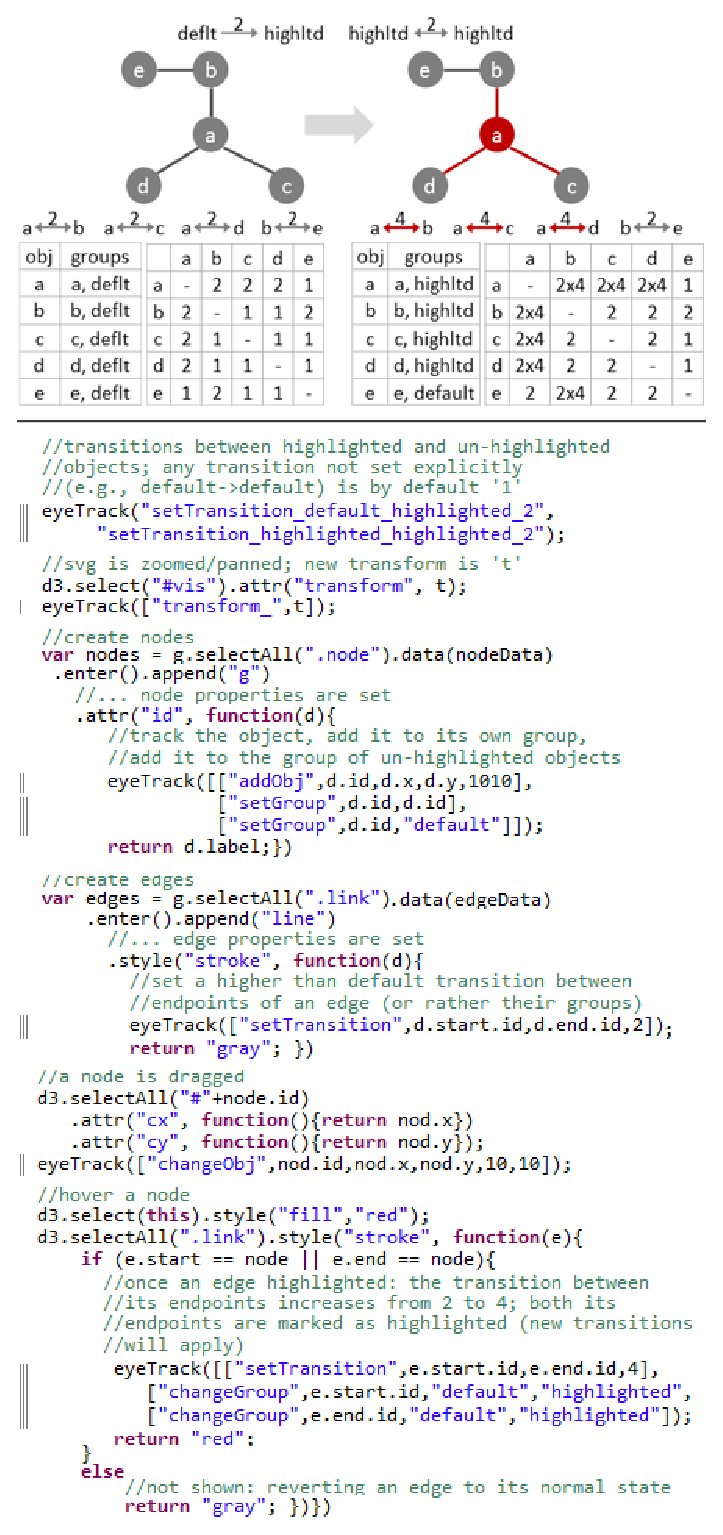
\includegraphics[width=1.\linewidth]{images/receipe.eps}
  \caption{Instrumenting a D3 graph visualization. (Top) Changing transition-probabilities at run-time. Selecting a node marks it and its direct neighbors as highlighted; transitions between these nodes, and from un-highlighted  nodes to these nodes, become more likely ($1\rightarrow2$), as do transitions on highlighted edges ($2\rightarrow4$). These rules translate to transitions between pairs of specific nodes; when multiple rules apply to a pair of nodes, their effects are compounded through multiplication. (Bottom) Three types of instrumentation calls mirror the visualization�s rendering and interaction code to capture: view changes ($|$), addition and updating of visual objects ($||$), and management of transition probabilities ($|||$).}
	\label{fig:snippets}
\end{figure}

Second, the library needed to know the positions and sizes of objects that the visualization drew on the screen. Instrumentation code was added to mirror instructions used to add, remove, and update visual objects. We note that this workflow integrates particularly well with the add-remove-update pattern of D3. 

Third, the library allowed visualizations to define transition probabilities between objects and manage them dynamically at run-time.  We achieved this by creating groups of objects  and specifying transition probabilities between those groups. Visual objects could be added or removed from a group, and transition probabilities between groups could change, at run-time. The top part of Figure 8 exemplifies the changes in transition probabilities once a user selects a node in a network visualization. 

Identifying and quantifying appropriate transition probabilities may be difficult for some visualizations, given that a solid understanding of how users parse and interpret visualizations does not yet exist. Our instrumentations relied on informal assumptions (e.g., a highlighted object is more likely to be viewed than an un-highlighted one) and follow the similar approach of Salvucci et al. We have also shown in section 4 that our assumptions held for the IMDB visualization we analyzed. A more principled way to determine typical viewing patterns and sequences in a specific visualization is to run a pilot study using no transition probabilities. Preliminary data could then be used to determine typical usage patterns and help refine viewed object detection by informing the choice of appropriate transition factors. Section~\ref{sec:Evaluation} shows how such an analysis could be done.
